\section{Modulo registro}

\subsection{Objetivo}
El objetivo de este módulo es poder registrar a nuevos usuarios dentro de la aplicación móvil, o para iniciar sesión en caso de que estos ya se encuentren registrados.

\subsection{Diseño}

Para éste módulo se desarrolló el inicio de sesión de la aplicación móvil, para ello fue utilizado el Inicio de Sesión con Apple ID provisto por Apple. Se eligió esta forma de autenticación ya que para poder acceder se deberá contar con un Apple ID, es decir, si no se cuenta con uno no se podrá accesar; de esta manera se asegura que los usuarios que se registren serán personas.

\subsection{Desarrollo}

Para el desarrollo fue necesario integrar \textit{ASAuthorizationAppleIDCredential} que es el encargado de proporcionar la información del Apple ID del usuario, en este caso fue solamente el nombre y el correo. Así mismo se implemento el botón \textit{ASAuthorizationAppleIDButton} que es el encargado de disparar la acción \textit{ASAuthorizationAppleIDProvider} para obtener la información del usuario. Cabe mencionar que para poder hacer uso completamente del Inicio de Sesión con Apple ID, se debe formar parte del \textit{Apple Developer Program}\footnote{Para más información ver: \url{https://developer.apple.com/programs/}}.


\subsection{Resultados}

La Figura \ref{fig:signin} muestra el resultado que se obtuvo por la implemetación del módulo de registro, en ella se puede ver como se integró el botón \textit{Sign in with Apple} provisto por Apple. \\

\begin{figure}[htbp]
	\begin{center}
		\fbox{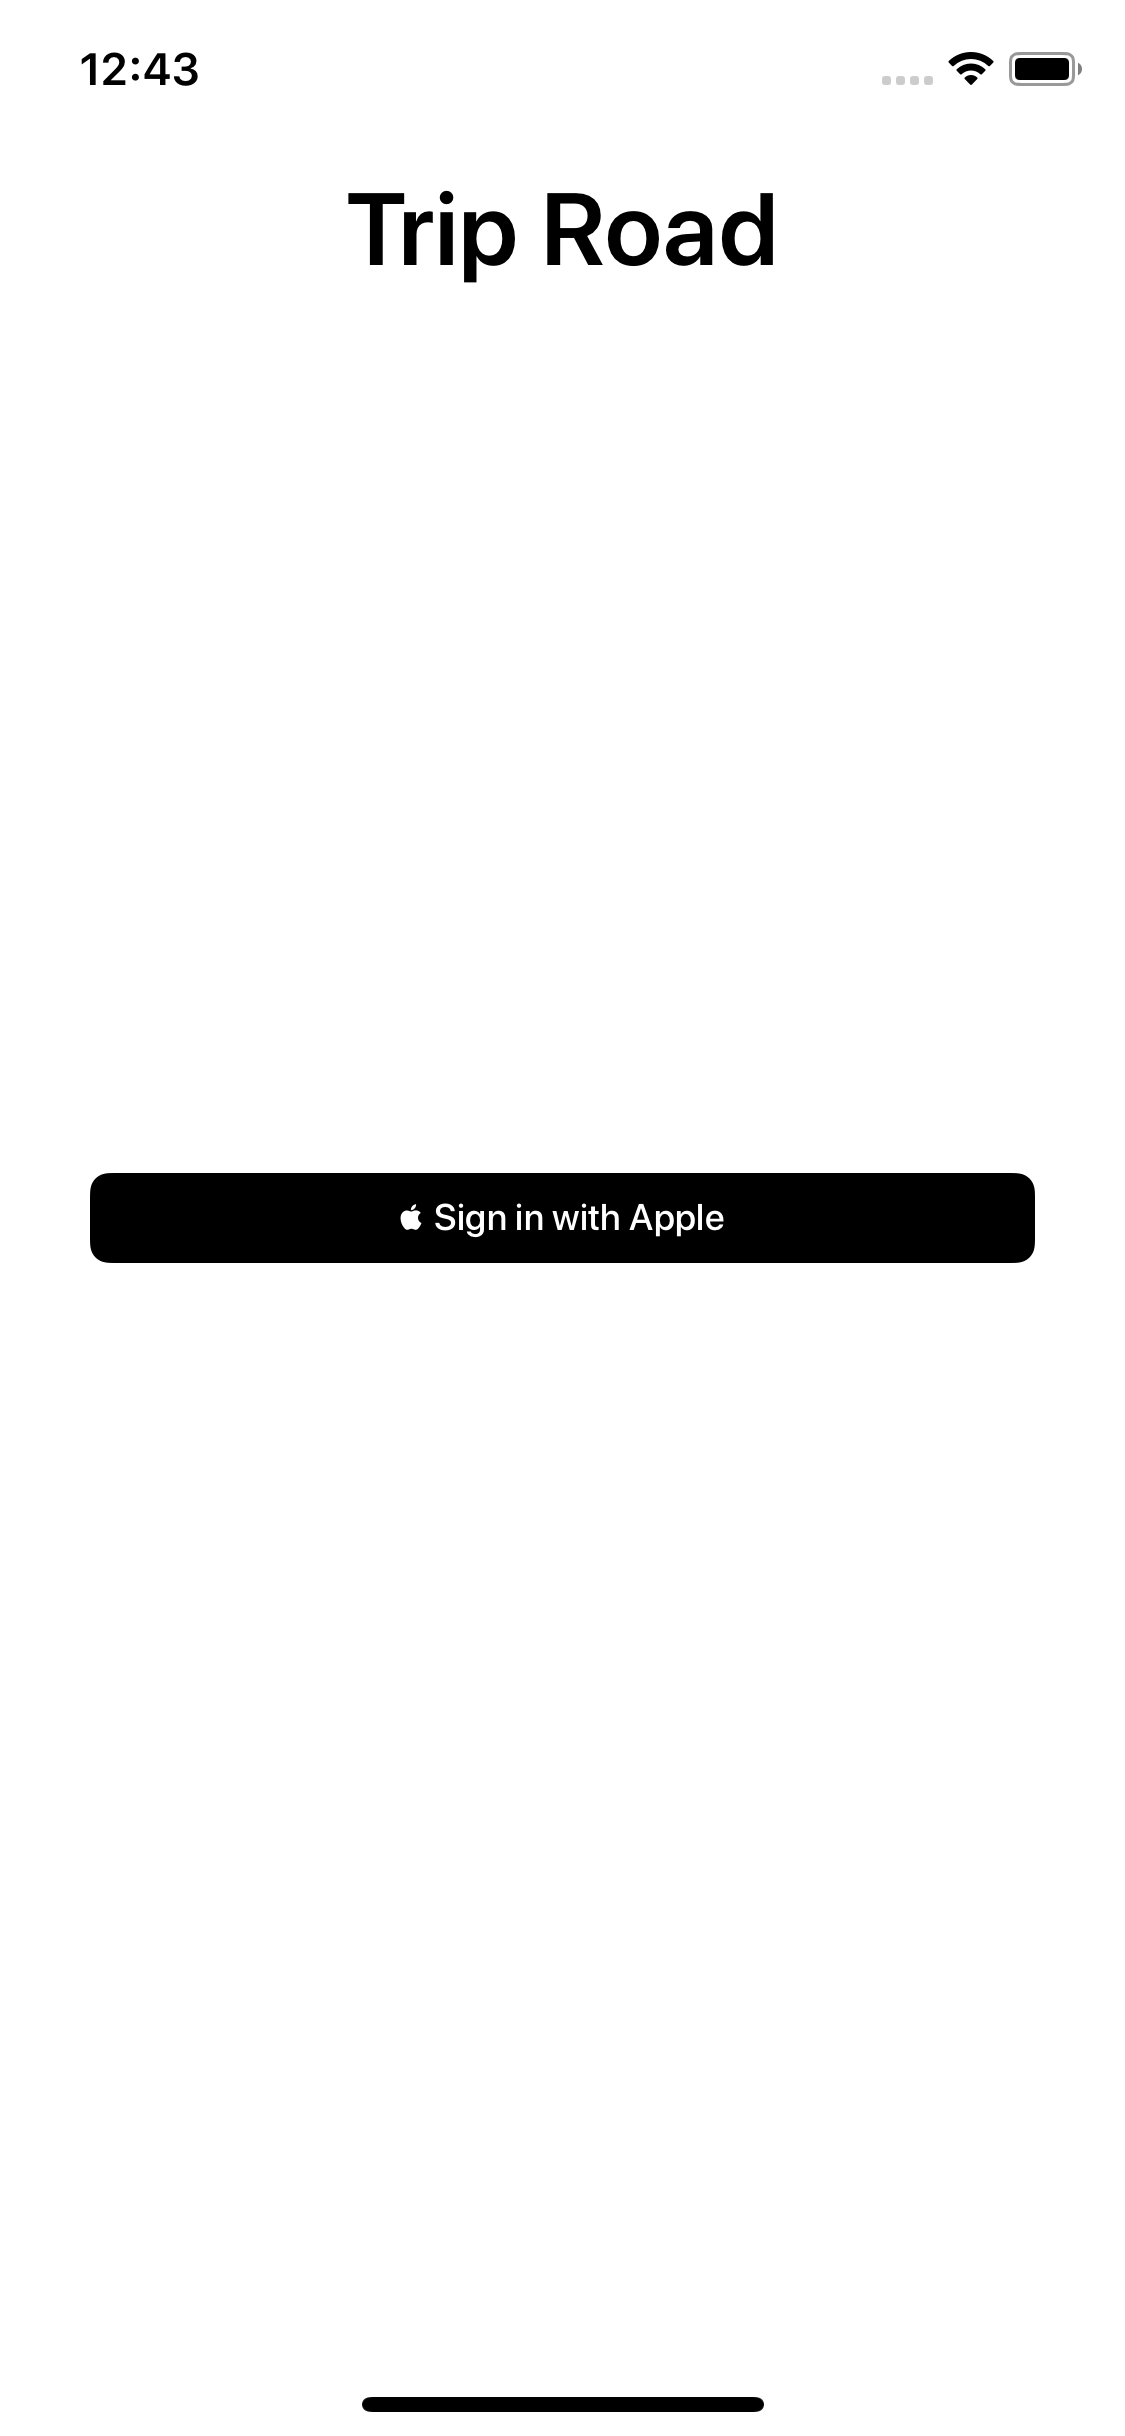
\includegraphics[scale = .1]{implementacion/registro/images/signin}}
		\caption{Resultado módulo registro}
		\label{fig:signin}
	\end{center}
\end{figure}


